\subsubsection{Descripción}

Frente a un problema, un algoritmo goloso va armando la solución global usando la heurística de eligir a cada paso la solución óptima local.
En general estos algoritmos son eficientes y simples de dise\~nar e implementar, pero puede ser que nunca lleguen a la soluci\'on \'optima global del problema. 

De acuerdo a la definici\'on de Brassard\footnote{\label{Brassard}Brassard G., Bratley P., {\it Fundamental of Algorithmics}, Prentice Hall, 1996. (c)}, un algoritmo goloso se compone de los siguientes elementos: 

\begin{enumerate}
 \item Un concepto de candidato, y una estructura de solución a partir de candidatos.
 \item Un conjunto de candidatos que ya han sido considerados y seleccionados. 
 \item Un conjunto de candidatos considerados y rechazados. 
 \item Una funci\'on que comprueba si cierto conjunto de candidatos constituye una soluci\'on a nuestro problema, ignorando si es o no \'optima por el momento. 
 \item Una funci\'on de factibilidad, que determina si es o no posible completar el conjunto a\~nadiendo otros candidatos para obtener al menos una soluci\'on de nuestro problema. 
 \item Una funci\'on de selecci\'on que indica en cualquier momento cu\'al es el m\'as prometedor de los candidatos restantes, que no han sido seleccionados ni rechazados. 
 \item Una funci\'on objetivo, que da el valor de la soluci\'on que hemos hallado. 
\end{enumerate}

\fixme{ver la correccion de estatico/dinamico}

Lo que busca el algoritmo goloso es encontrar la secuencia de candidatos que constituya una soluci\'on, y que optimice el valor de la funci\'on objetivo. Este algoritmo avanza paso a paso. Inicialmente, el conjunto de elementos seleccionados est\'a vac\'io. Entonces, en cada paso se considera a\~nadir a este conjunto el mejor candidato sin coniderar los restantes, de acuerdo a nuestra funci\'on selecci\'on. Si el conjunto ampliado de candidato seleccionados ya no fuera factible, rechazamo el candidato que estamos considerando en ese momento. Sin embargo, si el conjunto aumentado sigue siendo factible, entonces a\~nadimos el candidato actual al conjunto de candidatos selecccionados, en donde pasar\'a a estar desde ahora en adelante. Cada vez que se ampl\'ia el conjunto de candidatos seleccionados, comprobamos si \'este constituye ahora una soluci\'on para nuestro problema. A partir de este esquema, al agregar siempre soluciones \'optimas locales a mi conjunto, al finalizar lo que se espera encontrar es la soluci\'on \'optima global. 

El algoritmo de Dijsktra para encontrar caminos m\'inimos en un grafo pesado es un algoritmo goloso, que funciona y es correcto, como lo fue demostrado por Bassard et al. en el libro mencionado.

Dado un grafo $G=(V,X)$, Dijkstra guarda un conjunto $S$ de nodos que ya fueron recorridos y un vector $\pi$ con la distancia m\'inima encontrada de un nodo $u$ a todo el resto. Como invariante, el valor de $\pi$ de los nodos en $S$ ya es su distancia a $u$. En cada fase de Dijkstra, se selecciona un nuevo nodo de $V\backslash S$ cuyo valor en $\pi$ sea m\'inimo y se añade a $S$, actualizando si es necesario $\pi$. Al finalizar, $\pi$ es el vector con la m\'inima distancia a todos los nodos. 

Para resolver el problema se va a implementar Dijkstra con tres funciones objetivo diferentes, que toman una arista y devuelven un peso para ella: 

\begin{enumerate}
  \item $f_A(e) = \omega_1(e)$
  \item $f_B(e) = \omega_2(e)$
  \item $f_C(e) = \omega_1(e)\omega_2(e)$
\end{enumerate}

A continuación detallamos el pseudoc\'odigo de Dijkstra parametrizado para ejecutarse con distintas funciones de peso. La implementación utililza un heap para mantener la lista de nodos no visitados.

\begin{algorithm}
    \caption{\texttt{Dijkstra}}
In: Grafo $G = (V,X)$, nodo inicial $v_0$, ObjectiveFunction $f$ \newline
Out: Arreglo $\pi$ con camino m\'inimo en funci\'on de $f$ a cada nodo
\\Arreglo $previo$ con nodo anterior en el camino mínimo, para cada nodo
\begin{algorithmic}[1]
\State $\pi(v) = \infty$ \quad $\forall v \in V$
\State $previo(v) = null$ \quad $\forall v \in V$
\State $\pi(v_0) = 0$
\State $S = \emptyset$
\For{$i = 1 \dots n-1$}
    \State $v \leftarrow $ nodo de $V\backslash S$ de m\'inimo $\pi$. 
    \For{{\bf each} $w \in V\backslash S$ adyacente a $v$}
      \If{$\pi(v) + f((v,w))) < \pi(w)$}
        \State $\pi(w) = \pi(v) + f((v,w)))$
        \State $previo[w] \leftarrow v$
      \EndIf
    \EndFor
    \State $S = S \cup \{v\}$
\EndFor
\State \textbf{retornar} $\pi$, $previo$
\end{algorithmic}
\end{algorithm}

\begin{algorithm}
    \caption{\texttt{Reconstrucción del camino mínimo}}
\begin{algorithmic}[1]
    \State $path \leftarrow []$
    \State actual = $v$
    \While{$previo[actual] != null$}
        \State $path.push\_front(actual)$
        \State $actual \leftarrow previo[actual]$
    \EndWhile
    \State \textbf{retornar} path
\end{algorithmic}
\end{algorithm}

\newpage
\subsubsection{Complejidad}

De acuerdo al libro de Brassard antes mencionado, la complejidad de Dijkstra implementada sobre un heap es $O(m \log n)$. Se utilizó la implementación \texttt{priority\_queue} de la \textit{Standard Template Library} de $C++$ que garantiza la complejidad de heap\footnote{http://www.cplusplus.com/reference/queue/priority\_queue/priority\_queue/}. 

%-- Goloso A --
\clearpage
\subsubsection{Familias Malas - Greedy A: utiliza la función de peso $f_{A}$}\label{subsubsec:greedy-a}
Dado un grafo $G = (V,E)$, obtenemos el camino m\'inimo entre $u$ y $v$ seg\'un $\omega_1$. 

A continuación definimos una familia de grafos en los cuales nuestro algoritmo puede devolver resultados muy malos.
%\ponerGrafico{imagenes/maloGreedyA.png}{}{0.5}{malo-para-greedy-a}

\begin{figure}[H]
    \begin{center}
        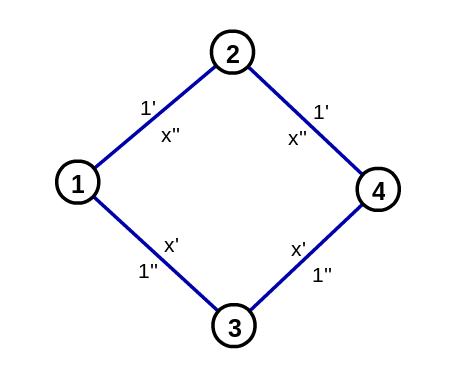
\includegraphics[scale=0.5]{imagenes/maloGreedyA.png}
        \caption{Familia de grafos malos para el Greedy A. En adelante, con un apóstrofe haremos referencia al peso por $\omega_1$ y con dos al peso por $\omega_2$}
    \end{center}
\end{figure}

Para ir de 1 a 4 hay dos caminos posibles: ($C_1$) $1 \rightarrow 2 \rightarrow 4$; ($C_2$) $1 \rightarrow 3 \rightarrow 4$

\begin{eqnarray}
 \omega_1(C_1) &=& 2 	\\ 
 \omega_2(C_1) &=& 2x	\\
 \omega_1(C_2) &=& 2x	\\
 \omega_2(C_2) &=& 2
\end{eqnarray}

Supongamos que K vale 2x, es decir, los dos caminos son válidos. Nuestro algoritmo elige $C_1$.
$\frac{\omega_2(C_1)}{\omega_2(C_2)} = x$.
Como x lo podemos variar, este cociente puede ser tan grande como queramos. Es decir que el algoritmo goloso puede devolver una solución
arbitrariamente alejada de la óptima.

El algoritmo puede encontrar una solución no factible. En ese caso, sa sabe que no existe una solución posible, ya que la solución encontrada tiene un valor por $\omega_1$ menor o igual al de cualquier otro camino.

%-- Goloso B --
\clearpage
\subsubsection{Familias Malas - Greedy B: utiliza la función de peso $f_{B}$}\label{subsubsec:greedy-b}
Dado un grafo $G = (V,E)$, obtenemos el camino m\'inimo entre $u$ y $v$ seg\'un $\omega_2$. 

A continuación definimos una familia de grafos en los cuales nuestro algoritmo puede devolver resultados muy malos.
\ponerGrafico{imagenes/maloGreedyB.png}{}{0.5}{malo-para-greedy-b}

Para ir de 1 a 4 hay dos caminos posibles: ($C_1$) $1 \rightarrow 2 \rightarrow 4$; ($C_2$) $1 \rightarrow 3 \rightarrow 4$

\begin{eqnarray}
 \omega_1(C_1) &=& 4 	\\ 
 \omega_2(C_1) &=& 2	\\
 \omega_1(C_2) &=& 2	\\
 \omega_2(C_2) &=& 2x
\end{eqnarray}

Supongamos que K vale 2. Nuestro algoritmo elige $C_1$, pero al no ser válido, se ve obligado a devolver ``no". Pero $C_2$ era una solución
válida. Ésto se cumple para cualquier valor de x.

Esta heurística, si devuelve una solución válida, entonces devuelve la solución óptima. Sin embargo, en cualquier instancia interesante de $CACM$ - que no se reduzca a encontrar el camino mínimo por $\omega_2$ - la heurística devolvería un camino inválido.

\clearpage
%-- Goloso C --
\subsubsection{Familias Malas - Greedy C: utiliza la función de peso $f_{C}$}\label{subsubsec:greedy-c}
Dado un grafo $G = (V,E)$, obtenemos el camino m\'inimo entre $u$ y $v$ seg\'un $\omega_1\omega_2$. 

Esta heurística se puede comportar de la misma forma que el Greedy B, si consideramos la familia mala de grafos desarrollada para el Greedy B,
restringiendonos a valores de x mayores a 2. Se eligiría $C_1$  para minimizar el producto de las funciones de peso. Como no es válido,
se deberá devolver ``no", a pesar de que $C_2$ era válido. 

\subsubsection{Conclusión: unificación de las tres heurísticas}
Las tres heurísticas \textit{GreedyA}, \textit{GreedyB} y \textit{GreedyC} no son muy útiles por separado. Se considerara la heurística \textit{Greedy} como:

\begin{algorithm}
    \caption{\texttt{Greedy}}
\begin{algorithmic}[1]
    \State $pathB \leftarrow GreedyB()$
    \If{$valido?(pathB)$}
        \State \textbf{retornar} pathB
    \EndIf
    \State $pathA \leftarrow GreedyA()$
    \State $pathC \leftarrow GreedyC()$
    \If{$valido?(pathC)$}
        \If{$\omega_2(pathA) < \omega_2(pathC$}
            \State \textbf{retornar} pathA
        \Else
            \State \textbf{retornar} pathC
        \EndIf
    \EndIf
    \If{$valido?(pathA)$}
        \State \textbf{retornar} pathA
    \Else
        \State \textbf{retornar} \texttt{no}
    \EndIf
\end{algorithmic}
\end{algorithm}

\subsubsection{Experimentación}
Resulta importante destacar las decisiones que tomamos para la generación de grafos. Nos cercioramos primero de que exista un camino entre $u$ y
$v$ que cumpla con la restricción de $k$. Luego fuimos agregando caminos, como para dar varias opciones a los algoritmos, con la particularidad
de que eran $balanceados$. Ésto significa que si el peso según $\omega_1$ del camino era bajo, entonces le asignábamos un $\omega_2$ alto.
Más aún, para todo camino $C$ entre $u$ y $v$, $\omega_1(C)$ y $\omega_2(C)$ estaban distribuidos simetricamente con respecto a $k$.
Es decir, el camino $P$ más corto según $\omega_2$ que cumpla con la restricción de $k$ era tal que $\omega_1(P)$ = $\omega_2(P)$ = $k$.
En particular, nosotros insertábamos este camino $P$ en el grafo, de modo que llevamos cuenta del valor de la solución óptima. Ésto nos va a
facilitar evaluar la calidad de una solución cuando la instancia es muy grande como para correr el backtracking.


\begin{figure}[H]
\begin{center}
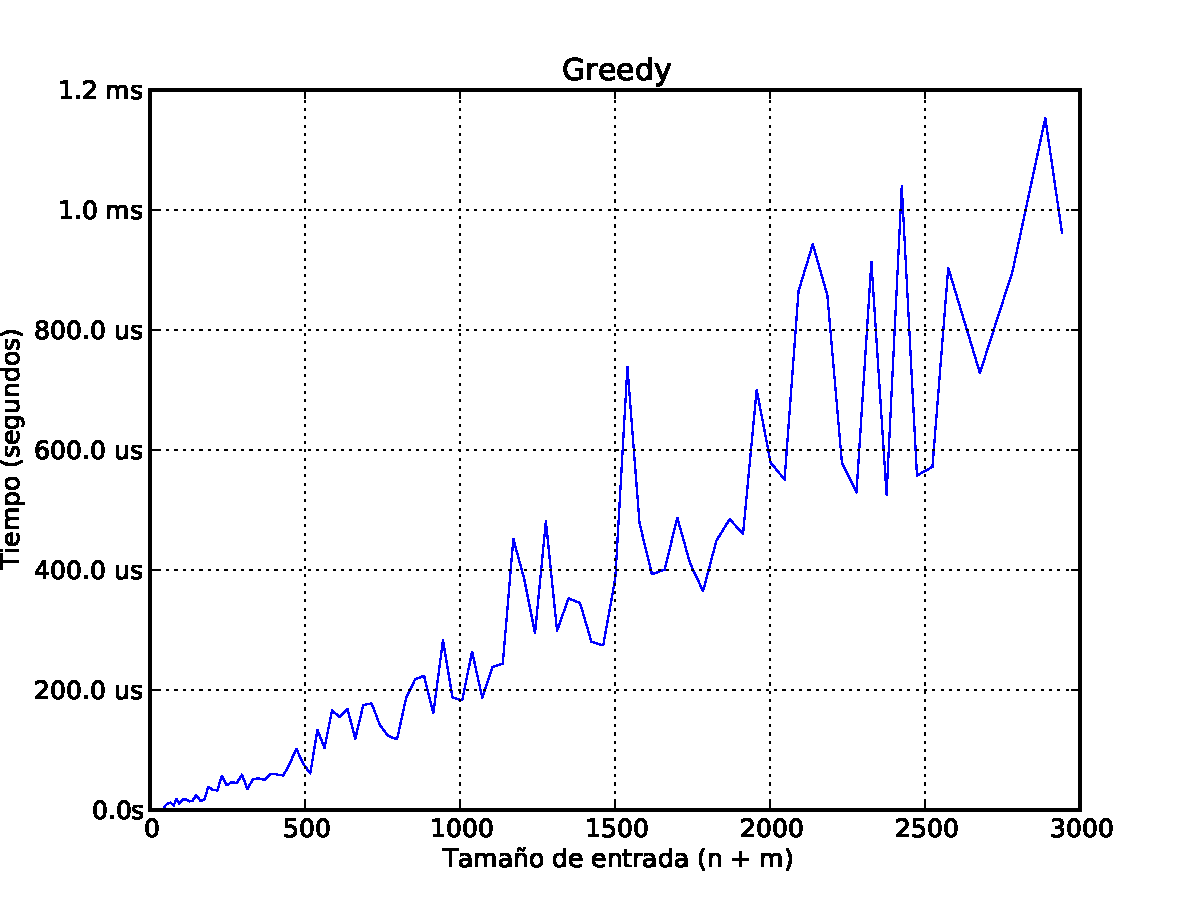
\includegraphics[angle=0, scale=.75]{imagenes/tiempos_greedy_magic_A.pdf}
\label{grafico local}
\end{center}
\end{figure}

Se puede interpretar la curva de tiempo de ejecución vs. tamaño de entrada como una función cercana a la lineal, aunque se puede percibir
que está ligeramente por encima de ésta.

\begin{figure}[H]
\begin{center}
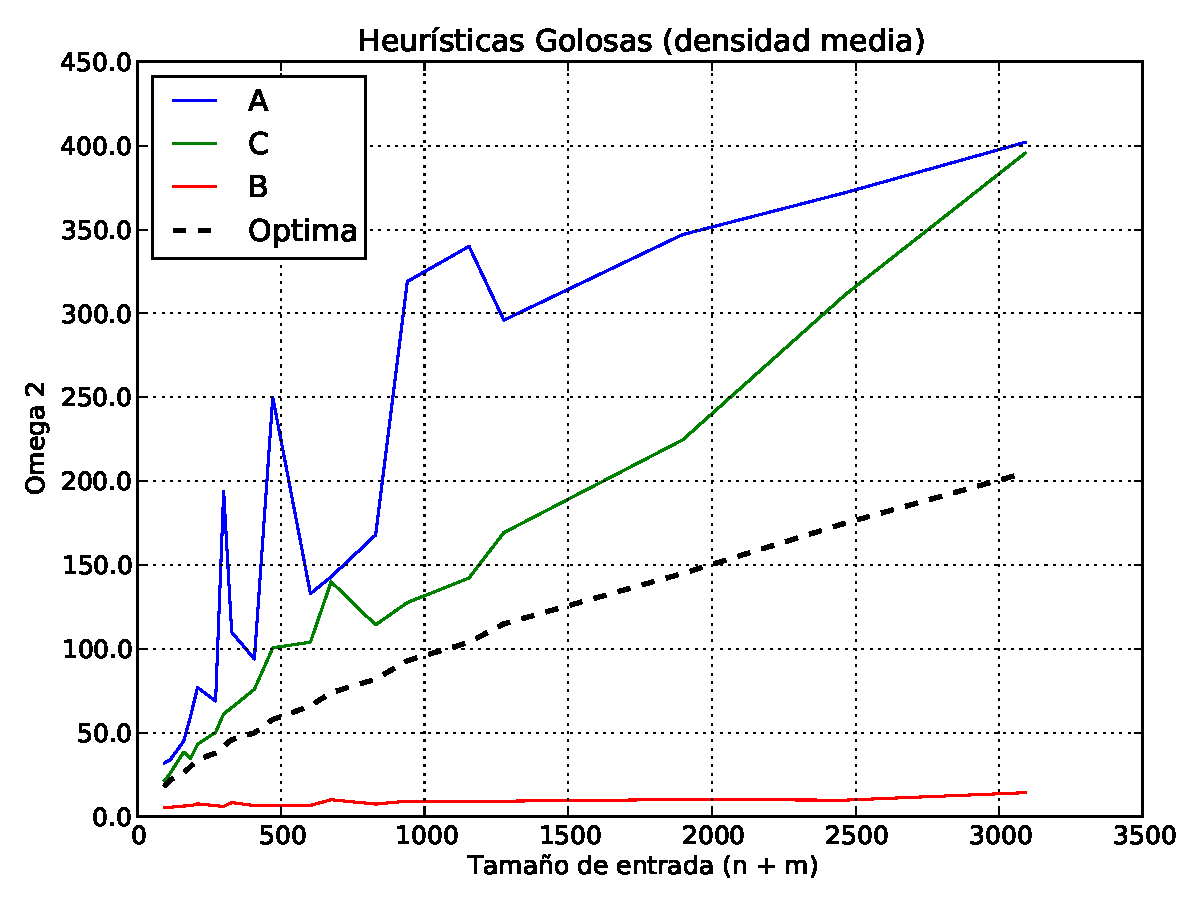
\includegraphics[angle=0, scale=.75]{imagenes/calidad_greedy_2014-06-27_09-50-48.pdf}
\label{grafico local}
\end{center}
\end{figure}

Lo que salta a simple vista es el bajo peso según $\omega_2$ de la heurística B. ¡Pareciera ser mejor solución que la óptima! Sin embargo,
recordando lo expuesto previamente, nos damos cuenta que si el peso según $\omega_2$ es menor que el de la óptima, entonces el peso según
$\omega_1$ es mayor que el de la óptima, es decir, que $k$. Por lo tanto no son soluciones válidas.
Ésto era de esperar - la heurística B sólo va construyendo su solución sin reparar siquiera en $\omega_1$.

Por otro lado tenemos la heurística A, que sólo mira $\omega_1$ y por lo tanto termina bastante alejada de la solución óptima. La heurística
C resultó ser un acierto, se acerca bastante a la solución válida, pero no descuida el mantenerse dentro de la cota de $k$.
